% !TeX spellcheck = it_IT

\section{Problemi di ottimizzazione}

Sono un caso particolare dei problemi come precedentemente definiti.\\

Un \textbf{problema di ottimizzazione} $\pi$: 
\begin{enumerate}
	\item \textbf{Input} $I_\pi \subseteq 2^\ast$
	
	\item Una \textbf{funzione} $Amm_\pi: \, I_\pi \rightarrow 2^{2^\ast} \setminus \{\emptyset\}$ \textbf{mappa} ogni \textbf{input} in un \textbf{insieme di soluzioni ammissibili}
	
	\item $c_\pi: 2^\ast \times 2^\ast \rightarrow \mathbb{N}$, $\forall x \in I_\pi$, $\forall y \in Amm_\pi (y)$, $c_\pi (x,y)$, ovvero un costo/guadagno, \textbf{funzione obiettivo}
	
	\item $T_\pi \in \{\max, \min\}$: "tipo del problema", voglio massimizzare o minimizzare il mio costo/guadagno
\end{enumerate}

\paragraph{Esempio:} Max-Sat
\begin{itemize}
	\item input: formule logiche in forma CNF, esempio:
	$$ (x_7 \vee x_2) \wedge (x_4 \vee \neg x_5 \vee \neg x_7) \wedge (x_9 \neg x_2) $$
	
	\item Le soluzioni ammissibili per una data formula $\varphi$ sono tutti gli assegnamenti delle variabili di di $\varphi$, quindi per l'esempio tutte le $2^5$ possibili combinazioni di assegnamenti delle $5$ variabili
	
	\item $c_\pi (\varphi, ass)$: il costo per ogni formula con un dato assegnamento è il numero di clausole rese vere dall'assegnamento
	
	\item $T_\pi = \max$: problema di massimizzazione, voglio un assegnamento che massimizzi il numero di clausole soddisfatte
\end{itemize}

Ovviamente non si può avere un algoritmo polinomiale che risolve questo problema in quanto sarebbe equivalente al CNF-SAT, avere il massimo numero di clausole soddisfacibili vorrebbe dire anche sapere se la formula è soddisfacibile.\\

\newpage

\subsection{Problema di decisione associato} 

Ad \textbf{ogni problema di ottimizzazione} $\pi$ \textbf{si può associare un problema di decisione} $\hat{\pi}$:
\begin{itemize}
	\item $I_{\hat{\pi}} = (x, k)$, $x \in I_\pi$, $k \in \mathbb{N}$.\\
	\item La risposta per l'input $(x,k)$ è sì iff $\exists y \in Amm_\pi (x)$ esiste una soluzione ammissibile tale che $c_\pi (x,y) \geq k$ per i problemi di massimizzazione, oppure $c_\pi (x,y) \leq k$ per problemi di minimizzazione (rientro nel costo $k$?).\\
\end{itemize}

Sostanzialmente, "trovare il minimo" diventa "esiste una soluzione con costo minore di $k$?".\\

\paragraph{Esempio:} per $\hat{\text{Max-Sat}}$
\begin{itemize}
	\item $I_{\hat{\text{Max-Sat}}} = \{ (\varphi, k) | \, \varphi$ formula CNF e $k \in \mathbb{N} \}$.\\
	\item $(\varphi, k)$ è \textit{sì} iff $\exists$ assegnamento che rende vere almeno $k$ clausole di $\varphi$.\\
\end{itemize}

\newpage

\subsection{Classe di complessità $\mathcal{PO}$}
Si definisce $\mathcal{PO}$ l'insieme dei problemi di ottimizzazione $\pi$ tali che $\pi$ è risolvibile in tempo polinomiale
$$ \mathcal{PO} = \{\pi \text{ problemi di ott. } | \, \pi \text{ risolvibile in t polinomiale } \}$$

\addcontentsline{toc}{subsubsection}{\protect\numberline{}Teorema}
\paragraph{Teorema:} Se $\pi \in \mathcal{PO}$, allora il suo problema di decisione associato sta in $\mathcal{P}$, i.e. $\hat{\pi} \in \mathcal{P}$.\\

\paragraph{Corollario:} Al contrario, se il problema di decisione associato $\hat{\pi}$ è $\mathcal{NP}c$, allora il problema non può essere risolto in tempo polinomiale $\pi \notin \mathcal{PO}$ (assumendo $\mathcal{P} \neq \mathcal{NP}$).\\

Esempio di problemi in PO: problemi di programmazione lineare. Mentre restringere il campo a solamente a soluzioni intere fa diventare il problema $\mathcal{NP}c$.\\

\newpage

\subsection{Rapporto di prestazione} 

Verranno trattati principalmente problemi che rientrano in $\mathcal{NP}c$, quindi non saranno risolvibili in modo esatto, ma solamente in modo approssimato. Ma come si quantifica l'approssimazione? \\

Dato un p.o. $\pi$, chiamiamo $\opt_\pi (x)$ il \textbf{valore ottimo della funzione obiettivo su input} $x$.\\
Dato un \textbf{algoritmo approssimato} $A$ (in input prende un possibile input ed in output fornisce una soluzione ammissibile, ma non necessariamente ottima) per $\pi$, definisco il \textbf{rapporto di approssimazione} 
$$ R_\pi (x) = \max \left\{\frac{c_\pi (x,y)}{opt_pi(x)}, \frac{opt_\pi (x)}{c_\pi (x,y)} \right\} $$
Il $\max$ serve a prendere un valore sempre $\geq 1$, sia per problemi di minimizzazione che massimizzazione, in modo da avere una definizione unica.\\

Si dice che $A$ è una \textbf{$\alpha$-approssimazione} per $\pi$ iff 
$$ \forall x \in I_\pi : \, R_\pi (x) \leq \alpha $$
Per ogni input $R_\pi (x)$ è minore o uguale di $\alpha$, sostanzialmente comunque vada quell'algoritmo non può essere peggio di $\alpha$ sul problema $\pi$. Ovviamente con $\alpha = 1$ l'algoritmo è esatto ed il problema sta in $\mathcal{PO}$.\\

\newpage

\subsection{Altre classi}
Si hanno altre possibili classi di problemi: 
\begin{itemize}
	\item Fuori da $\mathcal{PO}$ ($\mathcal{PO} \subset$), ci sono le classi \textbf{$n$-APX}, quindi $2$-APX ad esempio sono gli algoritmi che risolvono con $\alpha$ fino a 2 volte, 3 fino a 3 volte, ...; sostanzialmente classi sempre più grandi fino ad avere approssimazioni arbitrariamente grandi.\\
	
	\item \textbf{APX}: problemi risolvibili a meno di una costante di approssimazione di qualche tipo arbitrariamente grande, ma costante. Sempre algoritmi polinomiali, ma approssimati.\\
	
	\item Poi \textbf{$\log n$-APX}: approssimati ma l'approssimazione dipende anche dalla dimensione dell'input, fuori da APX (APX $\subset$).\\
	
	\item Tutte queste classi sono contenute in $\mathcal{NPO}$, ovvero l'equivalente di ottimizzazione di $\mathcal{NP}$.\\
	
	\item esistono anche problemi $\mathcal{NPO}$-completi $\mathcal{NPO}c$, ed interseca tutti i sottoinsiemi fin'ora (tranne $\mathcal{PO}$ ovviamente).\\
	
	\item \textbf{PTAS} (polinomial time approximation scheme), (appena fuori $\mathcal{PO}$): problemi approssimabili "quanto voglio", quindi posso decidere il tasso di approssimazione ma il tempo peggiora di conseguenza, anche in modo anche esponenziale.\\
	
	\item \textbf{FPTAS} (fully PTAS): dentro PTAS, fuori $\mathcal{PO}$, come PTAS, ma il tempo peggiora esclusivamente in modo polinomiale.\\
\end{itemize}

Dovrei mettere un disegnino con i cerchietti ma non ho assolutamente voglia, si capisce anche così dai (spero).\\

\newpage

% End of L2

\subsection{Problema di MaxMatching} 
Caratteristiche del problema: 
\begin{itemize}
	\item \textbf{Input:} un \textbf{grafo non orientato} $G = (V, E)$ e bipartito (due gruppi di nodi, i nodi all'interno di un gruppo non hanno collegamenti tra loro)
	\item \textbf{Soluzioni ammissibili:} chiamate \textbf{matching}, insieme $M$, una selezione di lati per cui nessun vertice incide su $>1$ lato, scegliere lati in modo da coprire il maggior numero di vertici possibili senza coprire nessun vertice più di una volta
	
	\item \textbf{Funzione obiettivo:} numero di lati scelti, ovvero \textbf{cardinalità di} $M$
	
	\item \textbf{Tipo:} problema di \textbf{massimizzazione} $= \max$, massimizzare il numero di vertici coperti
\end{itemize}

In questo caso la \textbf{soluzione ottima} si può trovare in \textbf{tempo polinomiale}, questo problema rientra in $\mathcal{PO}$. \\

\paragraph{Algoritmo del cammino aumentante:} un cammino aumentante viene definito su un grafo su cui è già presente un matching, anche parziale (solo in realtà, altrimenti non aumento nulla). Un \textbf{vertice} viene definito "\textbf{esposto}" quando su quel vertice \textbf{non incide nessun lato del matching}. \\

Un \textbf{augmenting path} è un \textbf{cammino} che \textbf{parte e arriva su un vertice esposto} ed \textbf{alterna lati} "liberi" (\textbf{non nel matching}) \textbf{e lati} "presi" (\textbf{nel matching}). Sequenza di lati alternata che inizia e termina su un vertice esposto. Partendo da vertici esposti il primo lato è per forza non preso.\\

Sapendo che c'è un cammino aumentante, è possibile scambiare i lati presi e non presi, si può fare uno \textbf{switch} sul cammino aumentante trovato. Partendo ed arrivando su nodi esposti per il cammino, \textbf{facendo lo switch} ci sarà sempre un \textbf{lato in più} "preso" \textbf{nel matching} e di conseguenza due nodi in più.\\

Se \textbf{ho un cammino aumentante posso migliorare il matching}, quindi quest'ultimo non è ottimo. Per migliorare il matching basta trovare un cammino aumentante, di conseguenza se lo trovo posso migliorare il matching, altrimenti il matching è massimo.\\

\paragraph{Lemma:} se \textbf{esiste un cammino aumentante} per il matching $M$, allora $M$ \textbf{non è massimo}.\\

\paragraph{Lemma 2:} se $M$ \textbf{non è massimo} allora \textbf{esiste un cammino aumentante}.\\

\begin{proof}
	Sia $M'$ un altro matching con $|M'| > |M|$ ($M$ non è massimo, ne esiste uno con cardinalità maggiore). Di conseguenza, considerando gli insiemi dei lati presi da ognuno dei matching, abbiamo tre zone tra i due insiemi: 
	\begin{itemize}
		\item lati in comune $M \cap M'$
		\item lati solo nell'insieme più piccolo $M \setminus M'$
		\item lati solo nell'insieme più grande $M' \setminus M$
	\end{itemize}
	
	Prendendo la differenza simmetrica tra i due
	$$ M \Delta M' = (M \setminus M') \cup (M' \setminus M)$$
	
	\textbf{Considerazione:} Nessun vertice può avere più di 2 lati coincidenti in $M \Delta M'$; se in ogni insieme possono avere un solo lato incidente ed ho due insiemi non possono essere più di 2 lati totali, il grado di ogni vertice sarà $\leq 2$, inoltre se ne ha 2 uno viene da un insieme ed uno dall'altro. \\ 
	Di conseguenza sul grafo generato dai lati in $M \Delta M'$ esiste $\exists$ almeno un cammino, composto da lati presi alternativamente uno da un insieme ed uno dall'altro, non possono essere di fila altrimenti vorrebbe dire che un vertice è stato considerato due volte all'interno dello stesso matching.\\
	Sapendo che $|M'| > |M|$ ci deve essere almeno un cammino che inizia e finisce con un lato di $M' \setminus M$ dato che sono di più e non può essere un ciclo (altrimenti sarebbero due lati dello stesso matching sullo stesso vertice). \\
	
	Essendo questo cammino alternanza di lati presenti in $M \setminus M'$ e lati in $M' \setminus M$ questo vuol dire che è un cammino aumentante per $M$.\\
\end{proof}

\newpage

%Questo è a prescindere dalle cose prima, serve per spiegare la roba dopo
\subsection*{Visite di grafi}
\addcontentsline{toc}{subsection}{\protect\numberline{}Visite di grafi}
Un po' estemporaneo ma serve spiegarlo.\\

Con "visite di grafi" si intende \textbf{metodi sistematici per "scoprire" un grafo}. Durante una visita i \textbf{nodi} possono rientrare in \textbf{3 categorie}:
\begin{itemize}
	\item sconosciuti, bianchi $W$ 
	\item conosciuti ma non visitati, grigi $G$, detti anche frontiera di visita
	\item visitati, neri $B$
\end{itemize}

La visita funziona iniziando \textbf{mettendo nella frontiera un solo nodo}, chiamato seed della visita. 
$$ F \leftarrow \{x_{seed}\}$$

Quindi in questo momento il nodo seme è grigio, tutti gli altri bianchi.
\begin{algorithm}
	\caption{VisitaGrafo ($Graph$)}
	\begin{algorithmic}
		\STATE $\forall x$ $c(x) \leftarrow W$
		\STATE $F \leftarrow \{x_{seed}\}$
		\STATE $c (_{seed}) \leftarrow G$
		\WHILE{$F \neq \emptyset$}
		\STATE $x \leftarrow $ pick$(F)$
		\STATE visit $x$
		\STATE $c(x) \leftarrow B$
		\FOR{$i \in $ neighbor$(x)$}
		\IF{$c(y) == W$}
		\STATE $F \leftarrow F \cup \{y\}$
		\STATE $c(y) = G$
		\ENDIF
		\ENDFOR
		\ENDWHILE
	\end{algorithmic}
\end{algorithm}

\newpage

Quando la frontiera è non-vuota, prendo un nodo dalla frontiera e visito questo nodo (qualunque cosa significhi). Coloro questo nodo di nero. Guardo tutti i vicini di questo nodo e:
\begin{itemize}
	\item se sono neri, già visitati, oppure grigi, già conosciuti, li lascio lì
	\item se sono bianchi li metto nella frontiera e li coloro di grigio
\end{itemize}

Per un grafo orientato l'unica cosa che cambia è scegliere se visitare i vicini uscenti o entranti (collegati con archi uscenti o entranti).\\

Se il \textbf{grafo è connesso} questo \textbf{garantisce di visitare ogni vertice una volta sola}. Se non è connesso verrà visitata solo la parte connessa del seme, per continuare serve un altro seed.\\

In base a \textbf{come viene scelto il nodo da prendere nella frontiera cambia il tipo di visita}, ad esempio con uno stack viene una DFS, con una coda viene una BFS, ma in generale, in base a come viene implementata la scelta del nodo si ha un tipo di visita diversa.\\

\newpage

\subsubsection{Trovare un cammino aumentante}
Un cammino aumentante deve \textbf{iniziare e terminare su un nodo esposto}, partendo da un grafico ed un matching. \\

Come \textbf{trovo nodi esposti}? faccio, partendo da ogni nodo \textbf{una BFS che alterna lati all'interno di} $M$ \textbf{e lati al di fuori di} $M$.\\

Se \textbf{una BFS} ad un certo punto \textbf{trova altri nodi esposti} allora abbiamo un \textbf{cammino aumentante}, altrimenti si passa alle BFS sul prossimo nodo, se \textbf{non viene trovato nessun altro nodo esposto} in nessun nodo allora \textbf{non ci sono cammini aumentanti}.\\

\begin{algorithm}
	\caption{FindAugmenting(G,M)}
	\begin{algorithmic}
		\STATE $X \leftarrow$ vertici esposti in $M$
		\FOR{all $x \in X$}
		\STATE  BFS$(x)$ con alternanza di lati $\notin M$ e $\in M$
		\ENDFOR
	\end{algorithmic}
\end{algorithm}

\paragraph{Tempo:} la BFS richiede tempo proporzionale al numero di lati $O(N \cdot M)$, una BFS per ogni vertice esposto, quindi al massimo $O(n^2)$. Quante volte dobbiamo eseguire FindAugmenting? al limite $n/2$, quindi $O(n/2 \cdot n^2) \subset O(n^3)$.\\

\addcontentsline{toc}{subsubsection}{\protect\numberline{}Teorema}
\paragraph{Teorema:} BipartiteMaxMatching $\in \mathcal{PO}$.\\

\paragraph{Corollario:} il problema di decisione PerfectMatching (il grafo ammette un matching massimale) è $\in \mathcal{P}$.\\

\newpage

Perché la BFS non funziona su grafi non bipartiti?
\begin{center}
	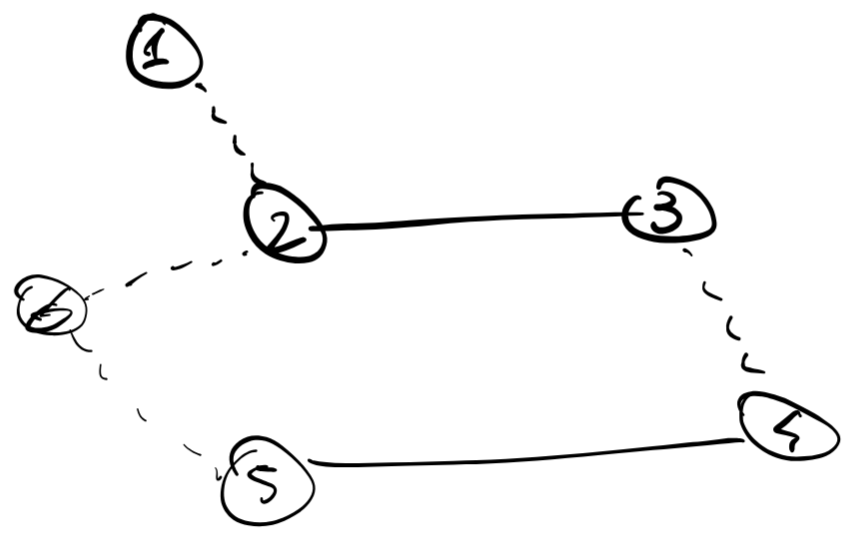
\includegraphics[width=0.8\columnwidth]{img/bipartito1}
\end{center}
Partendo da qualsiasi nodo esposto in questo grafo non si possono trovare cammini aumentanti (prova a farci la BFS alternata se non mi credi, stronzo (non ho voglia di scriverla)).\\

\newpage
